\documentclass{article}

\usepackage[a4paper]{geometry}
% \geometry{left=3cm,right=3cm,top=3cm,bottom=3cm}

\usepackage{graphicx}
\usepackage{subcaption}

\usepackage{mathtools}
\usepackage{amssymb}

\usepackage{minted}
\setminted[haskell]{escapeinside=@@}
\newcommand{\hs}{\mintinline{haskell}}

\usepackage[hidelinks]{hyperref}
\usepackage[utf8]{inputenc}
\usepackage{enumitem}

\usepackage[
backend=biber
]{biblatex}
\addbibresource{bibliography.bib}

\usepackage{isabelle,isabellesym}

\newcommand*{\term}[1]{{\isaspacing\isastyle \input{#1}}}
\newcommand*{\Term}[1]{{\isaspacing\isastyle #1}}
\newcommand*{\mTerm}[1]{\text{\Term{#1}}}

\renewcommand{\epsilon}{\varepsilon}
\newcommand{\eps}{\epsilon}
\newcommand{\overlay}{\oplus}
\newcommand{\connect}{\rightarrow}

\DeclarePairedDelimiter\abs{\lvert}{\rvert}%
\DeclarePairedDelimiter\norm{\lVert}{\rVert}%

\let\subsectionautorefname\sectionautorefname
\let\subsubsectionautorefname\sectionautorefname

% Swap the definition of \abs* and \norm*, so that \abs
% and \norm resizes the size of the brackets, and the 
% starred version does not.
\makeatletter
\let\oldabs\abs
\def\abs{\@ifstar{\oldabs}{\oldabs*}}
% 
\let\oldnorm\norm
\def\norm{\@ifstar{\oldnorm}{\oldnorm*}}
\makeatother

\title{Algebraic Graphs with Class}
\author{
  Christoph Madlener\\
  \texttt{\href{mailto:madlener@in.tum.de}{madlener@in.tum.de}}
}

\begin{document}

\maketitle
\begin{abstract}
  We give an overview of algebraic graphs as introduced by
  Mokhov~\cite{mokhov2017algebraic}. Algebraic graphs have a small and safe core
  of construction primitives, alongside a set of axioms, characterizing an
  algebra of graphs. They can be used to elegantly implement a graph
  transformation library employing functional programming. We also review the
  suitability of algebraic graphs for formal verification using Isabelle/HOL.
\end{abstract}

\section{Introduction}\label{sec:intro}
Graphs are a fundamental structure studied in depth by both mathematicians and
computer scientists alike. One very common definition states that a (directed)
graph is a tuple $G = (V,E)$, where $V$ is a set of vertices and $E \subseteq V
\times V$ is the set of edges. While this is a perfectly valid and natural
mathematical definition it is not necessarily suitable for implementation. This
can be illustrated by trying to directly translate this to Haskell:
\begin{minted}{haskell}
  data G a = G { vertices :: Set a, edges :: Set (a,a)}
\end{minted}
The value \hs{G [1,2,3] [(1,2),(2,3)]} then represents the graph $G =
(\{1,2,3\}, \{(1,2),(2,3)\})$, however \hs{G [1,2] [(2,3)]} does not
represent a consistent graph, as the edge refers to a non-existent node.
The state-of-the-art \texttt{containers} library implements graphs with
adjacency lists employing immutable arrays~\cite{king1995dfs}. The
consistency condition $E \subseteq V \times V$ is not checked statically though,
which can lead to runtime errors. \texttt{fgl}, another popular Haskell graph
library uses inductive graphs~\cite{erwig2001inductive}, also exhibiting partial
functions and potential for runtime errors due to the violation of consistency.

This led Mokhov to conceive \textit{algebraic
  graphs}~\cite{mokhov2017algebraic}, a sound and complete representation for
graphs. They abstract away from graph representation details and characterize
graphs by a set of axioms. Algebraic graphs have a small safe core of graph
construction primitives and are suitable for implementing graph transformations.
The four construction primitives are the following:
\begin{enumerate}
\item the \emph{empty} graph
\item single \emph{vertex} graphs
\item \emph{overlay}ing two graphs
\item \emph{connect}ing two graphs
\end{enumerate}
Overlay is the union of two graphs while connect also adds
edges from all vertices from one graph to all vertices of the other. 

Alongside proper definitions for these primitives we will see
in~\autoref{sec:locale} that this is indeed a sound and complete graph
representation. We will also cover the algebraic structure (\ref{sec:algebra})
exhibited by these graphs and elegant graph transformations (\ref{sec:trafo})
based on a type class for the core. In~\autoref{sec:verification} we explore how
we can exploit the algebraic structure in verification using Isabelle/HOL.

In~\autoref{sec:deep} we will examine the \emph{deep embedding} of the construction
primitives into an inductive datatype and its
applicability in practice and in verification (\ref{sec:quotient}). 

In~\autoref{sec:conclusion} we conclude and give an outlook on possible future
work and open questions connected to algebraic graphs as presented.

\section{A Type Class for Algebraic Graphs}\label{sec:locale}
This section will cover most parts of the original paper by
Mokhov~\cite{mokhov2017algebraic}. The graph construction primitives of
algebraic graphs will be formally defined and their soundness and completeness
proven. Afterwards we will cover the algebraic structure exhibited by these
primitives when interpreted as graphs. As part of this we will introduce a type class in Haskell which
further abstracts from implementation details. We will also see that different
classes of graphs can be obtained by modifying the axioms. Instances of
these different classes and a graph transformation library in Haskell are
presented. To conclude this section we will explore the suitability of this type
class for formal verification in Isabelle/HOL.

\subsection{The Core}\label{sec:core}
Before defining the four graph construction primitives we define the set of
graphs $\mathcal{G}$ over a fixed universe of vertices $\mathbb{V}$. A graph $G
\in \mathcal{G}$ can be represented as a tuple $G=(V,E)$ where $V \subseteq
\mathbb{V}$. A graph is \emph{consistent} if $E \subseteq V \times V$ holds.

The construction primitives
then are defined as follows. The \textit{empty} graph, denoted by $\eps$, is
simply the tuple $(\emptyset, \emptyset)$ which is clearly consistent, hence
$\eps \in \mathcal{G}$. Graphs with a single \textit{vertex} $v \in
\mathbb{V}$ and no edges, i.e.\ $(\{v\}, \emptyset)$, denoted by just $v$, are also
trivially consistent, hence $v \in \mathcal{G}$. The binary operations
\textit{overlay} and \textit{connect}, denoted by $\overlay$ and $\connect$
respectively, allow constructing larger graphs. Their definitions are
\begin{align*}
  (V_1, E_1) \overlay (V_2, E_2) &\coloneqq (V_1 \cup V_2, E_1 \cup E_2)\\
  (V_1, E_1) \connect (V_2, E_2) &\coloneqq (V_1 \cup V_2, E_1 \cup E_2 \cup V_1 \times V_2)
\end{align*}
So overlay is just the union of two graphs, while connect also adds an edge from
each vertex of its first argument to each vertex of its second argument. It is
straightforward to see that if $G_1 \in \mathcal{G}$ and $G_2 \in \mathcal{G}$
are consistent, then so are $G_1 \overlay G_2 \in \mathcal{G}$ and $G_1 \connect
G_2 \in \mathcal{G}$. In combination with the consistency of $\eps$ and of single vertex
graphs this already proves that algebraic graphs are a consistent
representation for graphs, i.e.\ using the construction primitives only yields
consistent graphs. The completeness of this representation, i.e.\ for
each $G \in \mathcal{G}$ there is an algebraic graph expression representing it,
is shown shortly (\ref{sec:algebra}). Both of these facts were also formally proven in
Isabelle/HOL (see~\autoref{sec:verification}).

As we will shortly see in~\autoref{sec:algebra} overlay and connect are somewhat
related to addition and multiplication in a semiring, hence, we give connect a
higher precedence
than overlay. Let us consider a few examples to develop some intuition for the
primitives. In these examples the universe of vertices are the natural numbers
and they are illustrated in~\autoref{fig:construction}.
\begin{enumerate}[label=(\alph*)]
\item $1 \overlay 2 = (\{1,2\}, \emptyset)$
\item $1 \connect 2 = (\{1,2\}, \{(1,2)\})$
\item $1 \connect (2 \overlay 3) = (\{1,2,3\}, \{(1,2), (1,3)\})$
\item $1 \connect 2 \overlay 2 \connect 3 = (\{1,2,3\}, \{(1,2), (2,3)\})$
\end{enumerate}
\begin{figure*}
  \centering
  \begin{subfigure}[b]{0.3\linewidth}
    \centerline{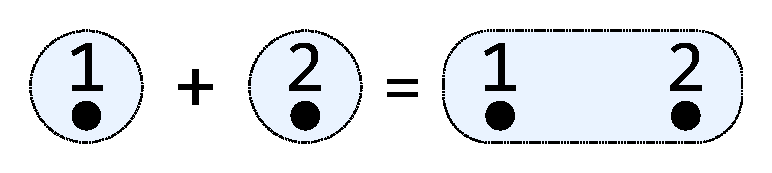
\includegraphics[scale=0.27]{fig/ex-a.pdf}}
    \vspace{-2.4mm}
    \caption{$1 \overlay 2$}
    \centerline{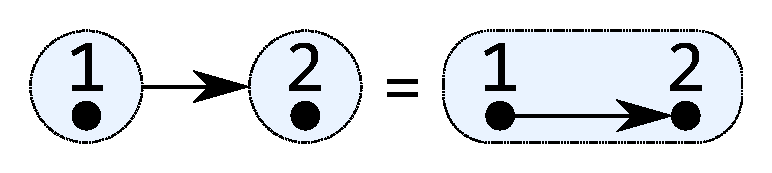
\includegraphics[scale=0.27]{fig/ex-b.pdf}}
    \vspace{-2.4mm}
    \caption{$1 \connect 2$}
  \end{subfigure}
  \begin{subfigure}[b]{0.3\linewidth}
    \centerline{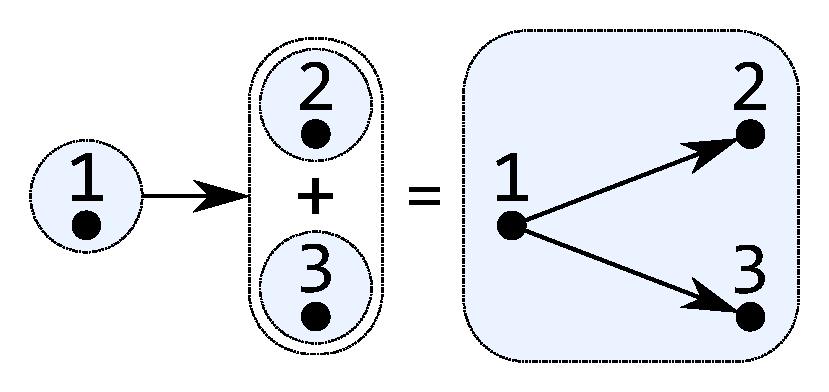
\includegraphics[scale=0.27]{fig/ex-c.pdf}}
    \vspace{-1mm}
    \caption{$1 \connect (2 \overlay 3)$}
  \end{subfigure}
  \hspace{3mm}
  \begin{subfigure}[b]{0.3\linewidth}
    \centerline{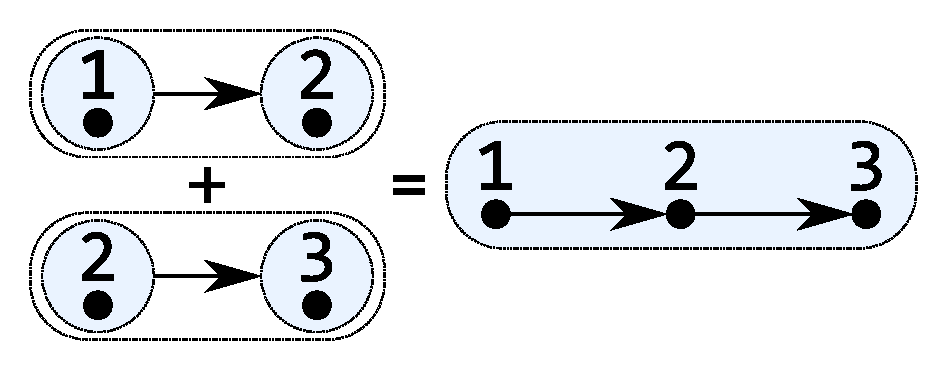
\includegraphics[scale=0.27]{fig/ex-e-new.pdf}}
    \vspace{-1mm}
    \caption{$1 \connect 2 \overlay 2 \connect 3$}
  \end{subfigure}
  \caption{Examples of graph construction. The overlay and connect operations
    are denoted by $\overlay$ and $\connect$, respectively. Illustrations
    from~\cite{mokhov2017algebraic}.\label{fig:construction}} 
\end{figure*}

We model the graph construction primitives in Haskell with the following type
class:
\begin{minted}{haskell}
  class Graph g where
      type Vertex g
      empty :: g
      vertex :: Vertex g -> g
      overlay :: g -> g -> g
      connect :: g -> g -> g
\end{minted}
The associated type \hs{Vertex g} represents the universe of vertices
$\mathbb{V}$, the remainder of the type class corresponds to $\eps$, single
vertex graphs, $\overlay$ and $\connect$ respectively.

At this point we will only introduce some very basic functions for constructing
graphs. More advanced constructions and transformations will be given
in~\autoref{sec:trafo}. A graph with a single edge is obtained by simply
connecting two vertices:
\begin{minted}{haskell}
  edge :: Graph g => Vertex g -> Vertex g -> g
  edge u v = (vertex u) `connect` (vertex v)
\end{minted}
A graph with only isolated vertices can be constructed from a list of vertices
as follows:
\begin{minted}{haskell}
  vertices :: Graph g => [Vertex g] -> g
  vertices = foldr overlay empty . map vertex
\end{minted}
Replacing \hs{overlay} with \hs{connect} in \hs{vertices} leads to a (directed)
clique. Later we will also consider undirected graphs. In that context this
function actually builds a fully connected graph on the given list of vertices.
\begin{minted}{haskell}
  clique :: Graph g => [Vertex g] -> g
  clique = foldr connect empty . map vertex
\end{minted}
Following and extending this approach leads to a safe and fully polymorphic
graph transformation library for any concrete graph representation (e.g.\ graphs
in \texttt{containers} or \texttt{fgl}) instantiating this class.

\subsection{Algebraic Structure}\label{sec:algebra}
Before turning to more advanced graph constructions we will observe the
algebraic structure of the primitives. It turns out that overlay and connect
almost form a semiring over graphs:
\begin{itemize}
\item $(\mathcal{G}, \overlay, \eps)$ is an idempotent, commutative monoid
\item $(\mathcal{G}, \connect, \eps)$ is a monoid
\item $\connect$ distributes over $\overlay$
\end{itemize}
For a proper semiring an annihilating zero for $\connect$ (i.e.\
$x \connect 0 = 0 = 0 \connect x$) is missing. It is also unusual that the two operations
share their identity $\eps$.

In addition there is the following
\textit{decomposition law}, as illustrated in~\autoref{fig:axioms}(b).
\[
  x \connect y \connect z = x \connect y \overlay x \connect z \overlay y \connect z
\]
\begin{figure*}
  \begin{subfigure}[b]{0.4\linewidth}
    \centerline{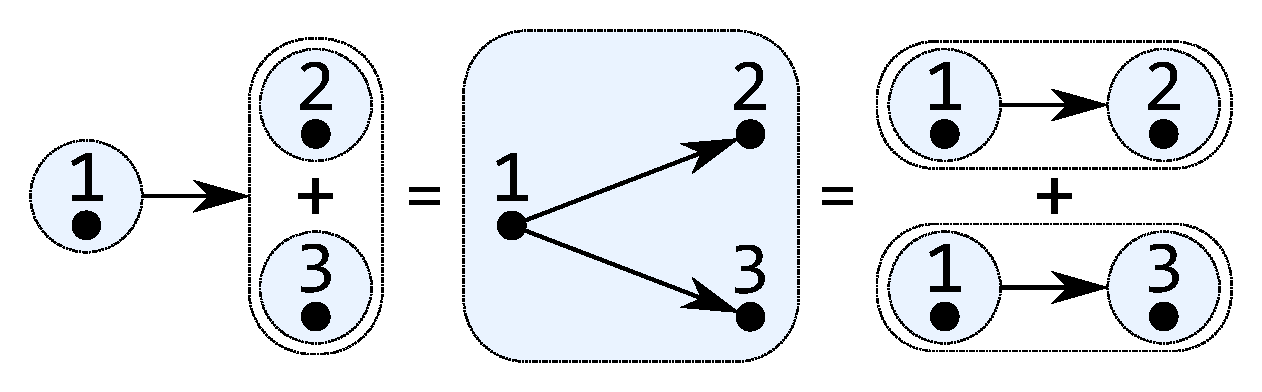
\includegraphics[scale=0.24]{fig/ax-distributivity.pdf}}
    \caption{Distributivity: $1 \connect (2 \overlay 3) = 1 \connect 2 \overlay
      1 \connect 3$ }
  \end{subfigure}
  \hspace{12mm}
  \begin{subfigure}[b]{0.5\linewidth}
    \centerline{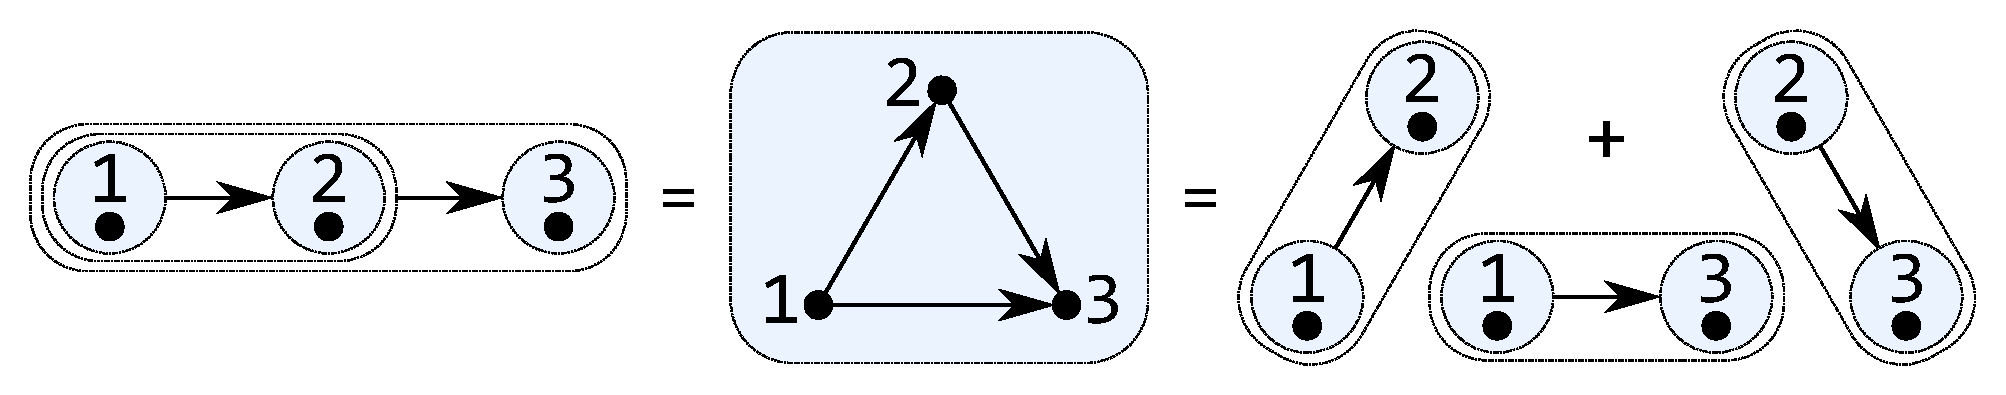
\includegraphics[scale=0.24]{fig/ax-decomposition.pdf}}
    \caption{Decomposition: $1 \connect 2 \connect 3 = 1 \connect 2 \overlay
      {1 \connect 3} \overlay {2 \connect 3}$}
  \end{subfigure}
  \vspace{-1mm}
  \caption{Two axioms of the algebra of graphs. Illustrations from~\cite{mokhov2017algebraic}.\label{fig:axioms}}
\end{figure*}
With decomposition we can prove by equational reasoning that $\overlay$ is
idempotent and that $\eps$ is indeed its identity.
According to Mokhov, the remaining axioms are a minimal set of axioms
\emph{characterizing} algebraic graphs~\cite{mokhov2017algebraic}. From the
original paper it does not become clear what he means by characterization:
Letting $\mathcal{G} = \{1\}$, $\eps = 1$, $1 \overlay 1 = 1$ and
$1\connect 1 = 1$ gives a structure abiding all axioms. This definition of
$\mathcal{G}$ is clearly not (isomorphic to) what we call directed graphs for
any universe of vertices.
We don't know which additional axioms are required to obtain this isomorphism.
However, the statement $\eps \neq vertex\ u$ for any $u \in \mathbb{V}$ does not
follow from the given axioms. Hence, adding an axiom scheme $\forall u \in
\mathbb{V}: \eps \neq vertex\ u$ seems sensible. Additionally $vertex$ probably
needs to be injective (i.e.\ $vertex\ u = vertex\ v \implies u = v$), however, we don't know if this
is sufficient.

One can, however, easily verify that the definitions of the primitives given
in~\autoref{sec:core} satisfy these axioms. At this point let us consider the
completeness of algebraic graphs. For any graph $G=(V,E)$ the following function
builds it using the four construction primitives:
\begin{minted}{haskell}
  graph :: Graph g => [Vertex g] -> [(Vertex g, Vertex g)] -> g
  graph vs es = overlay (vertices vs) (edges es)
\end{minted}
The \hs{edges} function generalizes \hs{edge} to a list of edges:
\begin{minted}{haskell}
  edges :: Graph g => [(Vertex g, Vertex g)] -> g
  edges = foldr overlay empty . map (uncurry edge)
\end{minted}
They are a direct translation of the fact, that any algebraic graph expression
$g$ for a graph $G=(V,E) \in \mathcal{G}$ can be rewritten in the 
\textit{canonical form}:
\[
  g = \left( \bigoplus_{v \in V} v \right) \oplus \left( \bigoplus_{(u,v) \in E}
  u \connect v \right)
\]

Mokhov also follows a standard approach of defining a partial order $(\preceq)$ for the
idempotent overlay operation as $x \preceq y \vcentcolon\Leftrightarrow x \overlay y = y$. This is indeed
a partial order under the graph axioms (i.e.\ it is reflexive, antisymmetric and
transitive). In fact this partial order can be used as a definition for
the subgraph relation, denoted by $\subseteq$:
\[
  x \subseteq y \vcentcolon\Leftrightarrow x \preceq y \vcentcolon\Leftrightarrow x \overlay y = y
\]

So far we only considered directed graphs. Undirected graphs can be
obtained from the very same construction primitives as directed graphs. It suffices
to modify the underlying axioms. In the case of undirected graphs this can be
achieved by making connect commutative (then denoted by $\leftrightarrow$),
i.e.\ adding the axiom $x \leftrightarrow y = y \leftrightarrow x$. By
introducing this axiom we can prove some of the other axioms of directed graphs.
Hence, according to Mokhov~\cite{mokhov2017algebraic}, undirected graphs are
characterized by the following minimal set of axioms:
\begin{itemize}
\item $(\mathcal{G}, \oplus)$ is a commutative semigroup
\item $\leftrightarrow$ is commutative and has $\eps$ as the identity
\item left distributivity: $x \leftrightarrow (y \oplus z) = x \leftrightarrow
  y \oplus x \leftrightarrow z$
\item left decomposition: $(x \leftrightarrow y) \leftrightarrow z = x
  \leftrightarrow y \oplus x \leftrightarrow z \oplus y \leftrightarrow z$
\end{itemize}
By choosing different additional axioms, other classes of graphs can be
characterized. Some examples are reflexive graphs (i.e.\ each vertex has a
self-loop), transitive graphs (as used in dependency graphs), and the combination
thereof; preorders. Combining undirected graphs and reflexive graphs yields
equivalence relations. It is even possible to define hypergraphs of arbitrary
(but fixed) rank by replacing the decomposition law with another suitable
axiom~\cite{mokhov2017algebraic}. In all of these the same caveats regarding the
term \emph{characterization} from directed graphs apply.

In summary the algebraic approach to graph representation has a small and safe
core of construction primitives. Pairing these primitives with suitable sets of
axioms leads to a highly flexible representation for graphs.

\subsection{Graph Transformation Library}\label{sec:trafo}
Based on the core type class, Mokhov implements what he refers to as a graph
transformation library\footnote{Algebraic graphs on hackage:
  \texttt{\href{http://hackage.haskell.org/package/algebraic-graphs}{http://hackage.haskell.org/package/algebraic-graphs}}}.
In order to understand the following constructions and transformations better,
we follow his approach and first define instances for the type class
\hs{Graph}. Recall the attempt from the introduction to directly translate the
graph representation $G=(V,E)$ into the Haskell datatype \hs{G}. We will now
define a \hs{Graph} instance for that datatype, while realizing that more
generally it can be used to represent relations on some domain (hence the renaming
to \hs{Relation}).
\begin{minted}{haskell}
  data Relation a = R { domain :: Set a, relation :: Set (a, a)} deriving Eq

  instance Ord a => Graph (Relation a) where
    type Vertex (Relation a) = a
    empty       = R Set.empty Set.empty
    vertex  x   = R (singleton x) Set.empty
    overlay x y = R (domain x `union` domain y) (relation x `union` relation y)
    connect x y = R (domain x `union` domain y) (relation x `union` relation y `union`
      fromAscList [ (a, b) | a <- elems (domain x), b <- elems (domain y) ])
\end{minted}
Mokhov also defines a \hs{Num} instance for \hs{Relation} which enables the use
of \hs{+} and \hs{*} as shortcuts for \hs{overlay} resp.\ \hs{connect}.

The given \hs{Graph} instance for \hs{Relation} satisfies the axioms of directed
graphs, as was argued in~\autoref{sec:core}. Obtaining \hs{Graph} instances
which satisfy the axioms for undirected graphs (or other classes of graphs) is
also straightforward: One can simply wrap \hs{Relation} in a \hs{newtype} and
define a custom \hs{Eq} instance. An example for undirected graphs (in this case
the connection to symmetric directed graphs is very prominent) is given.
\begin{minted}{haskell}
  newtype Symmetric a = S (Relation a) deriving (Graph, Num)

  instance Ord a => Eq (Symmetric a) where
    S x == S y = symmetricClosure x == symmetricClosure y
\end{minted}
It is also sensible to introduce subclasses like \hs{class Graph g => UndirectedGraph g}
to reflect the class of graph we are working with in the type system, and thus,
increase type safety.

Equipped with these two instances let us now actually consider graph
constructions and transformations made possible with the core type class. Simple
examples include constructing a \textit{path} from a list of vertices, which
then can be easily extended to a \textit{circuit}:
\begin{minted}{haskell}
  path :: Graph g => [Vertex g] -> g
  path []  = empty
  path [x] = vertex x
  path xs = edges $ zip xs (tail xs)

  circuit :: Graph g => [Vertex g] -> g
  circuit [] = empty
  circuit xs = path (xs ++ [head xs])
\end{minted}
Mokhov also gives functions for constructing \textit{star} graphs (i.e.\ a
center vertex connected to a set of leaves) and for building graphs from
\hs{Tree}s and \hs{Forest}s from the \texttt{containers} library.

More interesting applications include the implementation of a zero time
graph transposition using yet another \hs{newtype}
wrapper~\cite{mokhov2017algebraic}:
\begin{minted}{haskell}
  newtype Transpose g = T { transpose :: g } deriving Eq

  instance Graph g => Graph (Transpose g) where
    type Vertex (Transpose g) = Vertex g
    empty       = T empty
    vertex      = T . vertex
    overlay x y = T $ overlay (transpose x) (transpose y)
    connect x y = T $ connect (transpose y) (transpose x)
\end{minted}
Although for certain representations it is possible to get an $\mathcal{O}(1)$
transpose operation (e.g.\ by setting a transposed flag), for many typical
representations the whole graph has to be traversed, resulting in
$\mathcal{O}(\abs{V} + \abs{E})$ time.

More sophisticated transformations can be implemented using the following
\hs{Functor}-like \hs{newtype} wrapper. The function \hs{gmap} takes a function
\hs{a -> b} and a graph with vertices of type \hs{a} and produces a graph with
vertices of type \hs{b}.
\begin{minted}{haskell}
  newtype GraphFunctor a = F { gfor :: forall g. Graph g => (a -> Vertex g) -> g }

  instance Graph (GraphFunctor a) where
    type Vertex (GraphFunctor a) = a
    empty       = F $ \_ -> empty
    vertex  x   = F $ \f -> vertex (f x)
    overlay x y = F $ \f -> overlay (gmap f x) (gmap f y)
    connect x y = F $ \f -> connect (gmap f x) (gmap f y)

  gmap :: Graph g => (a -> Vertex g) -> GraphFunctor a -> g
  gmap = flip gfor  
\end{minted}
Interestingly this can be used to merge vertices fulfilling some predicate
\hs{p} by mapping them to a single vertex:
\begin{minted}{haskell}
  mergeVertices :: Graph g => (Vertex g -> Bool)
    -> Vertex g -> GraphFunctor (Vertex g) -> g
  mergeVertices p v = gmap $ \u -> if p u then v else u
\end{minted}
In the original paper \hs{gmap} is then used further to construct rather
sophisticated graphs fully polymorphically~\cite{mokhov2017algebraic}, i.e.\
independent from any concrete graph representation.

Mokhov also goes on to introduce a \hs{Monad}-like \hs{newtype} wrapper. The
\hs{bind} function in the context of graphs allows to replace each vertex with a
(possibly empty) subgraph. This can be used to both remove and split vertices.
\begin{minted}{haskell}
  newtype GraphMonad a = M { bind :: forall g. Graph g => (a -> g) -> g }

  instance Graph (GraphMonad a) where
    type Vertex (GraphMonad a) = a
    empty       = M $ \_ -> empty
    vertex x    = M $ \f -> f x
    overlay x y = M $ \f -> overlay (bind x f) (bind y f)
    connect x y = M $ \f -> connect (bind x f) (bind y f)
\end{minted}
Removing a vertex with \hs{bind} can be generalized to a function \hs{induce},
which only keeps vertices satisfying some predicate \hs{p}.
\begin{minted}{haskell}
  induce :: Graph g => (Vertex g -> Bool) -> GraphMonad (Vertex g) -> g
  induce p g = bind g $ \v -> if p v then vertex v else empty
\end{minted}
Splitting a vertex works by replacing that vertex with a graph containing the
desired vertices.
\begin{minted}{haskell}
  splitVertex :: (Graph g, Eq (Vertex g)) => Vertex g -> [Vertex g] 
    -> GraphMonad (Vertex g) -> g
  splitVertex v vs g = bind g $ \u -> if u == v then vertices vs else vertex u
\end{minted}
Mokhov then defines yet another \hs{newtype} wrapper utilizing \hs{bind} to
remove edges. He also showcases the construction capabilities of the presented
library by constructing de Bruijn graphs (a rather sophisticated type of graph
occurring frequently in computer engineering and bioinformatics)
completely polymorphically. These definitions are omitted here for brevity.

The presented material on the given type class gives an overview of an elegant,
reusable and polymorphic graph construction and transformation library. Note
that in the available \texttt{hackage} library for algebraic graphs the
\hs{newtype} wrappers for graph transformation are not implemented as such.
Instead there is a higher-kinded type class which is based
on \hs{MonadPlus}, but has fewer instances~\cite{mokhov2017algebraic}.

\subsection{Verification}\label{sec:verification}
We have now seen how to implement a polymorphic graph transformation library in
Haskell using the core type class. Mokhov proposes that algebraic graphs and
their axiomatic characterization are suitable for formal verification as they
enable equational reasoning. Some
simple statements (like $\hs{vertices xs} \subseteq \hs{clique xs}$) are given
accompanied by an Agda formalization\footnote{available at
  \texttt{\href{https://github.com/snowleopard/alga-theory}{https://github.com/snowleopard/alga-theory}}}.
For the examples in that formalization the claim obviously holds.

To experiment further we first formalized the material from the paper in
Isabelle/HOL~\cite{isabelle}.
This formalization\footnote{available at
  \texttt{\href{https://github.com/cmadlener/algebraic_graphs}{https://github.com/cmadlener/algebraic\_graphs}}}
the definition of several \textit{locale}s. For the purposes of this paper a
locale be thought of as a type class which can be equipped with axioms. The
following locale is the basis for our formalization.

\vspace{3mm}
\term{terms/locale_primitives}
\vspace{3mm}\newline
Note that it does not have any
axioms, as we reuse it to define locales for different classes of graphs (i.e.\
directed, undirected, etc.). Proving the statements from the paper in Isabelle/HOL works
without problems.

Noschinski formalized fundamental aspects of graph theory in
Isabelle/HOL~\cite{GraphTheory-AFP}. Part of that is essentially the standard
representation of a graph as a tuple $G=(V,E)$ (i.e.\ a locale with one single
axiom ensuring consistency). Instantiating a locale in Isabelle/HOL (which can be likened to
instantiating a type class in Haskell) requires to prove the axioms attached to
it. Using the definitions from~\autoref{sec:core} for the primitives it is
straightforward to instantiate the algebraic graph locale for the tuple
representation. We also formally prove that the graph construction primitives only
produce consistent graphs. A proof for the completeness of the primitives is
given as well (in the sense that every graph represented by a tuple can be
obtained using the algebraic graph construction primitives).

As the statements in the original paper were of very limited scope, we 
define and reason about more \textit{advanced} graph theoretic concepts: We
introduce (vertex) walks and the notion of reachability on algebraic graphs. A
challenge posed by the approach is that a graph is simply a value of some
abstract type \Term{'g}. Thus, we characterize the existence of a vertex or an
edge in a given graph by the subgraph relation (denoted by $\sqsubseteq$ in the
formalization):

\vspace{3mm}
\term{terms/has_elem}
\vspace{3mm}\newline
Equipped with these definitions we can then go on to inductively define when a
list of vertices is a walk in a given graph:

\vspace{3mm}
\term{terms/vwalk_def}
\vspace{3mm}\newline
We define the empty list as well as the list containing only a single vertex of
the graph as walks (\Term{vwalk\_Nil} and \Term{vwalk\_single}). Additionally if
a list with head \Term{v} (note that Haskell's \hs{(:)} is denoted by \Term{(\#)} in
Isabelle) is a walk and $(u,v) \in E$, then prepending \Term{u} also yields a
walk. Now we can prove various statements about walks (e.g.\ appending walks,
splitting walks, etc.). Interestingly, many of these statements follow directly
from the inductive definition of walks, i.e.\ we don't require any of the
algebraic graph axioms to prove them. We only need them when a proof relies on
the fact that $(u,v) \in E$ implies $u \in V$ as well as $v \in V$ (in other
words, the consistency of a graph).

For reachability we took two approaches. First we defined the set of edges of a
graph as follows:

\vspace{3mm}
\term{terms/edge_set_def}
\vspace{3mm}\newline
Reachability then can be defined via the reflexive, transitive closure of the
edge set. The second approach is to say that $v$ is reachable from $u$ if and
only if there is a walk from $u$ to $v$. These are, however, only proof of
concepts as only transitivity of reachability has been shown for both definitions.

Nonetheless, first impressions from these experiments suggest that it is
feasible to base more sophisticated formalizations of graph theory on algebraic
graphs. We did not experiment with adding additional axioms as described
in~\autoref{sec:algebra}. We instantiate the locale with the unit type, where
all primitives simply map to the unit value. This formalizes that the current
set of axioms is insufficient.

Exploring verification using the locale further is an interesting direction for
future work. The Haskell type class forms the basis for a polymorphic graph
transformation library. In the same vein, the locale can be seen as a
\textit{polymorphic} graph formalization
library. Any lemma we can prove using the locale axioms becomes available to any
graph representation instantiating the locale. This obviously becomes more
interesting the more material is available in the locale. Haslbeck et al.\ chose
a similar approach to implement and verify Kruskal's algorithm independent of
the concrete graph representation~\cite{Kruskal-AFP}.

\section{Deep Embedding}\label{sec:deep}
Up until this point we were mainly concerned with exploiting the algebraic
structure of graphs for polymorphic graph constructions and transformations, and
for formal verification. However, the deep embedding of the
construction primitives in a datatype is interesting in itself. Recall the
definition from the introduction:
\begin{minted}{haskell}
  data Graph a = Empty
               | Vertex a
               | Overlay (Graph a) (Graph a)
               | Connect (Graph a) (Graph a)
\end{minted}
An instance for the type class can be defined easily, however, we cannot use the
derived \hs{Eq} instance for the datatype, as it would violate the graph axioms:
\hs{Overlay Empty Empty} and \hs{Empty} both represent $\eps$ but are not deemed
equal.
One solution is to fold the deep embedding into a concrete graph representation to
obtain a law-abiding \hs{Eq} instance:
\begin{minted}{haskell}
  fold :: Graph g => Graph (Vertex g) -> g
  fold Empty         = empty
  fold (Vertex  x  ) = vertex x
  fold (Overlay x y) = overlay (fold x) (fold y)
  fold (Connect x y) = connect (fold x) (fold y)

  instance Ord a => Eq (Graph a) where
    x == y = fold x == (fold y :: Relation a)
\end{minted}
This approach is also currently implemented in the library available on
\texttt{hackage} (although an adjacency map is used instead of a relation).
However, this is not ideal for multiple reasons. Coupling the datatype to some
other graph representation merely for equality checks is undesirable.

More interestingly algebraic graphs can compactly represent dense graphs.
Consider the graph \hs{clique [1..n]}, which has a linear size representation in
the deep embedding, while it is quadratic when stored as a \hs{Relation}.
Requiring to fully expand graphs to check equality voids this advantage. A
promising approach to alleviate this issue is \textit{modular graph
  decomposition}~\cite{mcconnell2005linear}, as it allows to minimize algebraic
graph expressions.

More interesting questions for future work come up in connection with the deep
embedding. Currently only the transformations presented with the type class, i.e.\
transpose, as well as anything that can be done using the corresponding versions
of \hs{gmap} and \hs{bind}, are implemented directly on the deep embedding. No
efficient implementations of fundamental graph algorithms - like
depth-first-search - that work directly on the deep embedding are
known~\cite{mokhov2017algebraic}. The current library implementation therefore
resorts to converting algebraic graph expressions to an adjacency map and reuses
existing algorithms on this representation.

One application that comes to mind is search. Consider a best case example,
where only a small part of a dense graph has to be expanded before finding a target:
This allows us to exploit the better space complexity (linear vs.\ quadratic)
while also being competitive regarding time. The neighborhood of a vertex in an
algebraic graph can be computed in linear (in the size of the graph expression)
time and space.

Benchmarks (on an earlier version of the library) were performed by Moine to compare
the performance of the deep embedding to \texttt{containers} and \texttt{fgl}
(and one other representation). The results vary heavily depending on the area of
application. In some cases algebraic graphs offer a competitive alternative,
while in others, they perform orders of magnitudes worse. For the full results
refer to the repository containing the benchmark suite\footnote{available at
  \texttt{\href{https://github.com/haskell-perf/graphs}{https://github.com/haskell-perf/graphs}}}.

\subsection{Verification}\label{sec:quotient}
We were also interested in using the deep embedding in formal verification using
Isabelle/HOL. Hence, we ported the functions to Isabelle/HOL and then proved
their correctness. This
turned out to be very convenient, as the inductive datatype definition of the deep
embedding enables proofs by induction. Many of the resulting subgoals were then handled
automatically by Isabelle.

In the Haskell implementation of the deep embedding we already saw that
structural equality does not satisfy the axioms. There we can define a custom
\hs{Eq} instance to obtain a law-abiding datatype. In Isabelle/HOL we can follow
a similar approach, which results in a \texttt{quotient\_type}, which can be
thought of as an equivalence class construction on the raw datatype. For the
moment the equivalence is based on conversion of algebraic graph expressions to
the tuple representation by Noschinski mentioned in~\autoref{sec:verification}.
Again, the minimization of algebraic graph expressions to obtain an equivalence
relation on algebraic graphs, decoupled from any other graph representation, is
very much desirable.

The quotient type also allows us to formally prove that it satisfies the axioms,
by instantiating the locale corresponding to the core type class. It also paves
the way for further formalization efforts on the deep embedding. However, this
also requires more work to become truly interesting, i.e.\ if algorithms that
work directly on the deep embedding or other advanced usages of it can be found.

\section{Conclusion}\label{sec:conclusion}
We saw a novel approach to representing graphs, which is especially suitable for
functional programming. It allows for safe, polymorphic and elegant graph
constructions and transformations. Algebraic graphs also lend themselves nicely
to formal verification.

The alert reader might have noticed that the given primitives can only be used
to represent unlabeled graphs. Mokhov extended the algebraic graph library to
also represent edge-labeled graphs. There is no published material on this yet
(besides the source code). For more information refer to the talk by Mokhov
during Haskell eXchange 2018\footnote{available at
  \texttt{\href{https://skillsmatter.com/skillscasts/12361-labelled-algebraic-graphs}{https://skillsmatter.com/skillscasts/12361-labelled-algebraic-graphs}}}.

Algebraic graphs as presented have been successfully used in practice, e.g.\ for
asynchronous circuit design~\cite{beaumont2017high} and acceleration of graph
processing using FPGAs~\cite{mokhov2019language}. In these examples
the available transformations are sufficient. An important direction for future
research is going beyond those (relatively simple) transformations. That means
to find and formulate algorithms either inside the core type class or directly
on the deep embedding. Berghammer et. al~\cite{berghammer2020relational}, as well
as, Guttmann and Robinson-O'Brien~\cite{Relational_Minimum_Spanning_Trees-AFP}
successfully employ algebraic approaches to formally verify graph algorithms.
However, they are using an algebra of relations as opposed to the one here
defined on graph construction primitives. Dolan~\cite{dolan2013fun} uses an
algebra on adjacency matrices (specifically a semiring) to find paths in graphs.
Mokhov himself postulates that the algebraic approach allows to formulate graph
algorithms as systems of equations with unknowns. This may also be an approach
for finding novel graph algorithms.

\printbibliography

\end{document}